% Five intact source photographs; edit panel labels and arrangement here.
\begin{figure*}[t]
\centering
\begin{minipage}[t]{0.192\textwidth}\centering
{\small\sffamily\bfseries (a) Desktop/Planar}\par\smallskip
\vbox to 91pt{\vfil\hbox to \linewidth{\hfil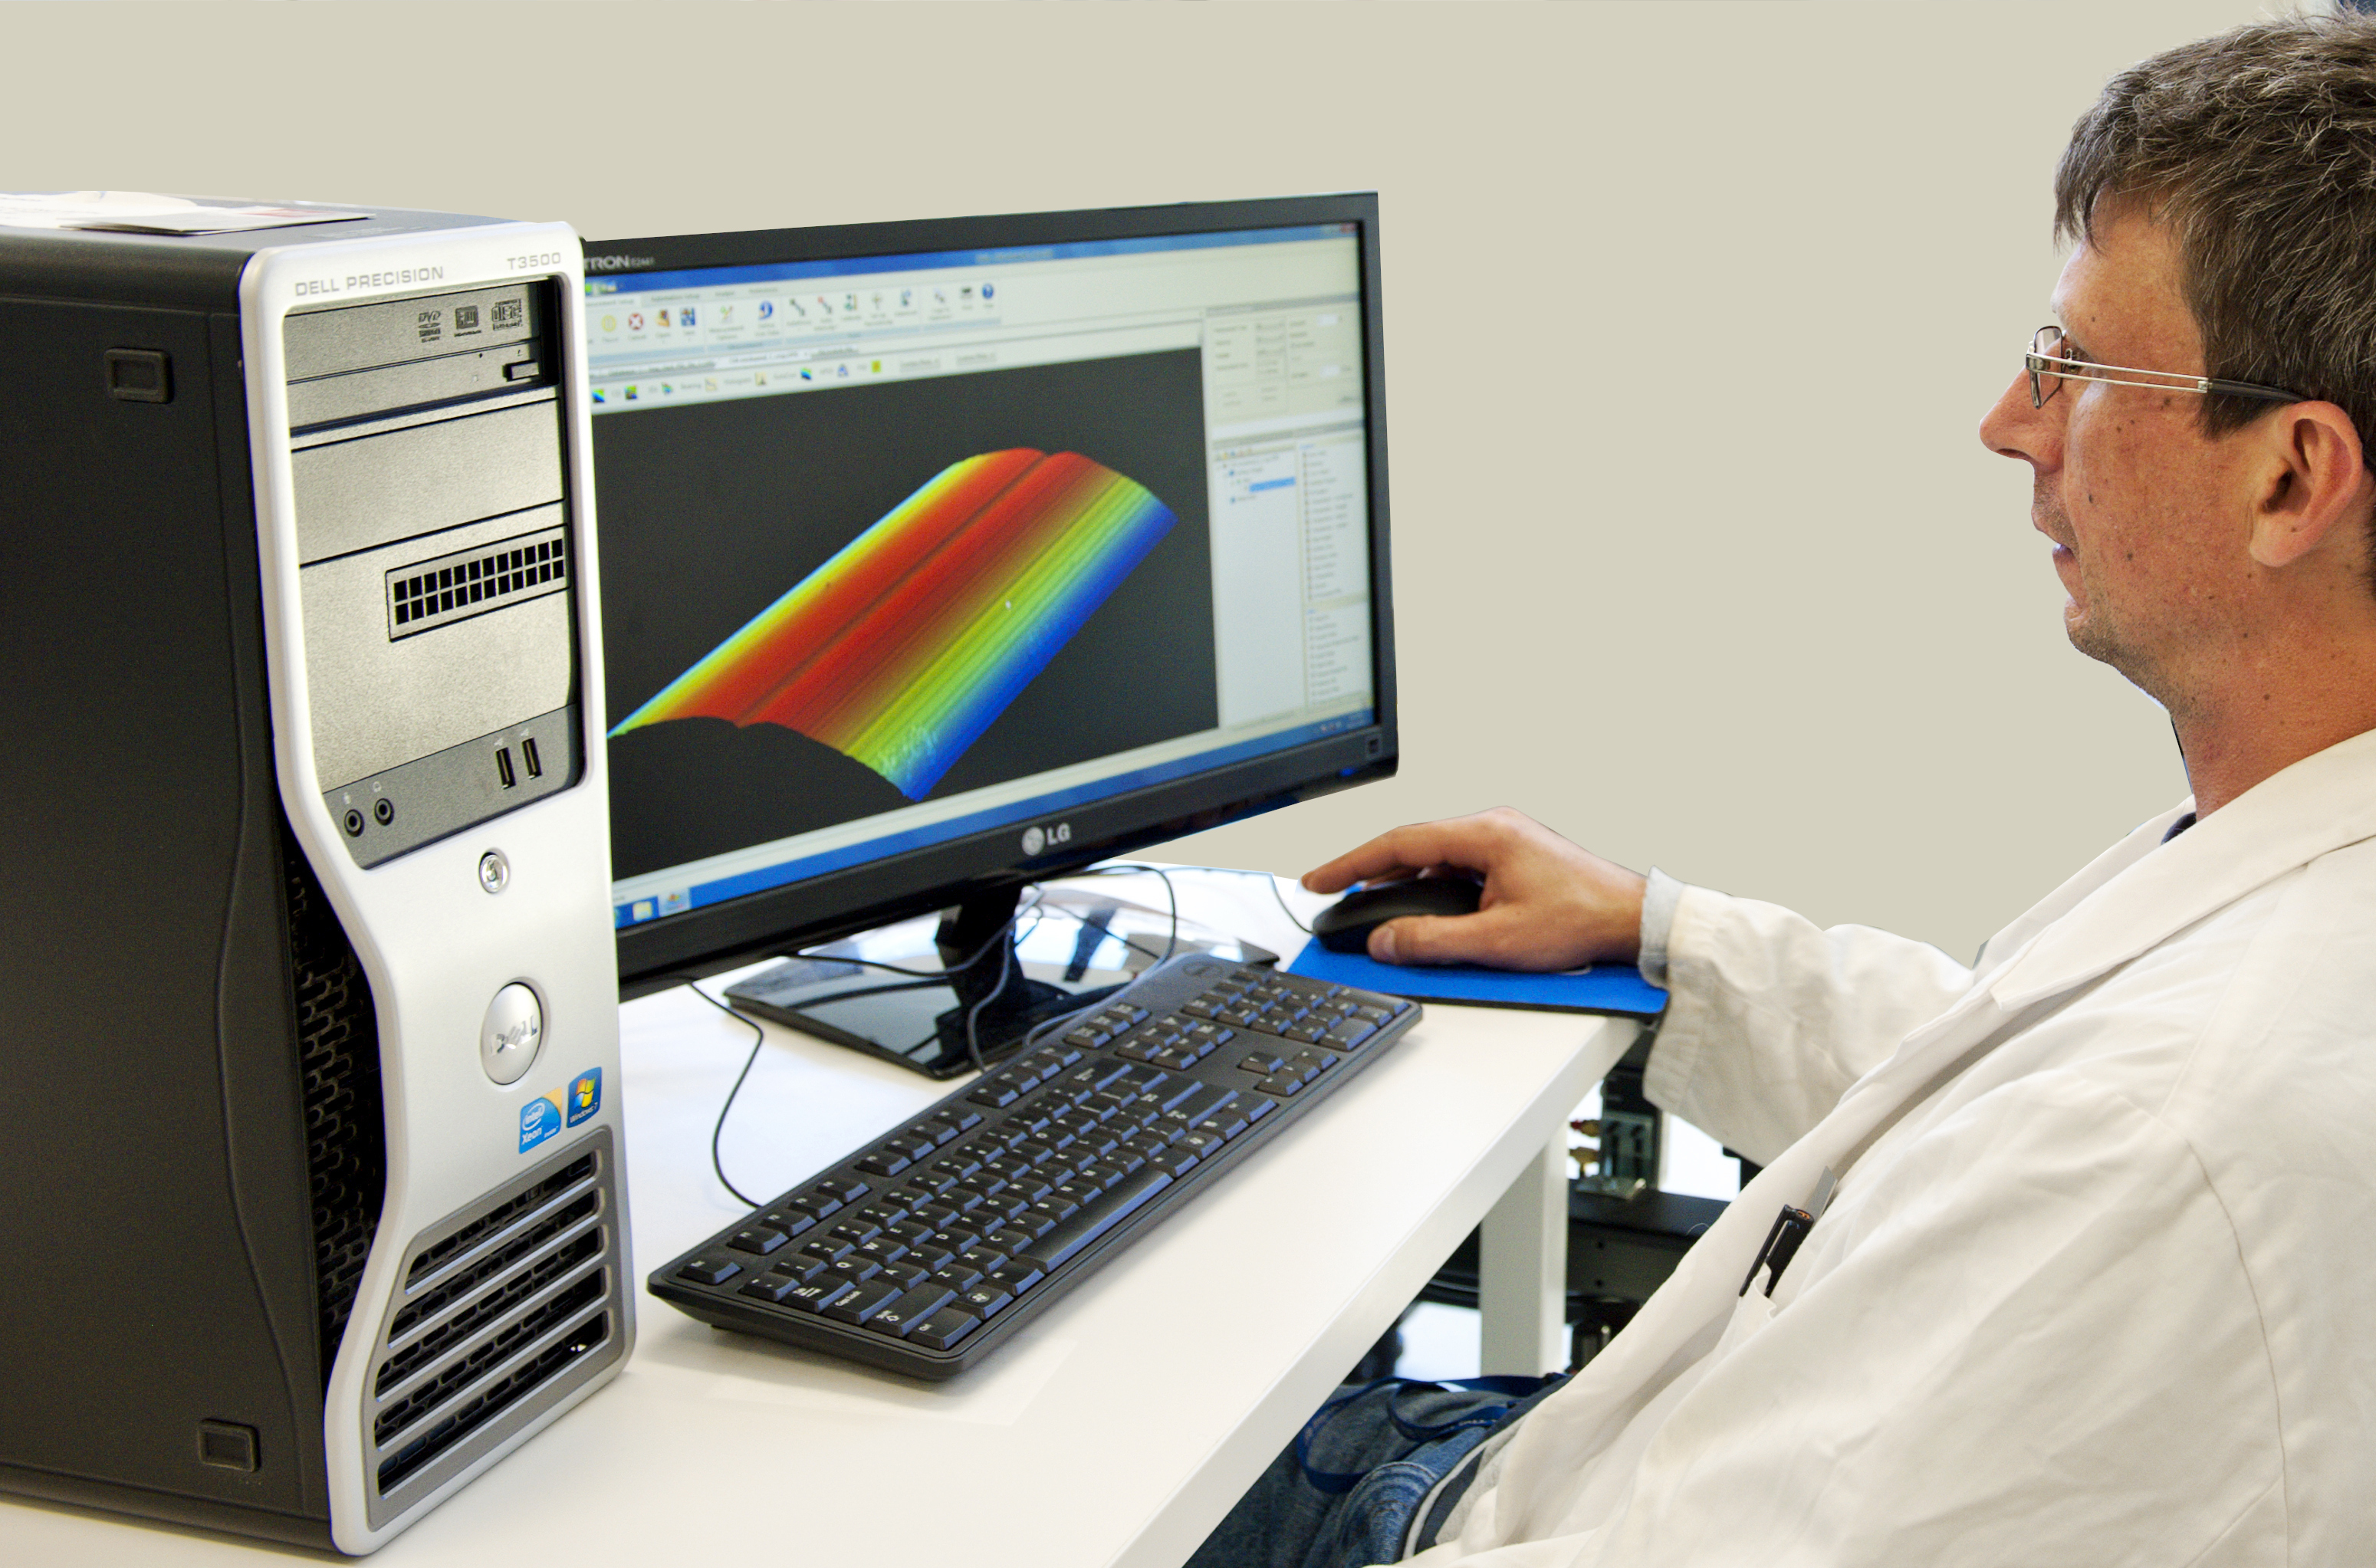
\includegraphics[width=\linewidth,height=91pt,keepaspectratio]{figures/desktop.jpg}\hfil}\vfil}
\smallskip{\scriptsize\sffamily Monitor-based views\par}
\end{minipage}\hfill
\begin{minipage}[t]{0.192\textwidth}\centering
{\small\sffamily\bfseries (b) Large Display}\par\smallskip
\vbox to 91pt{\vfil\hbox to \linewidth{\hfil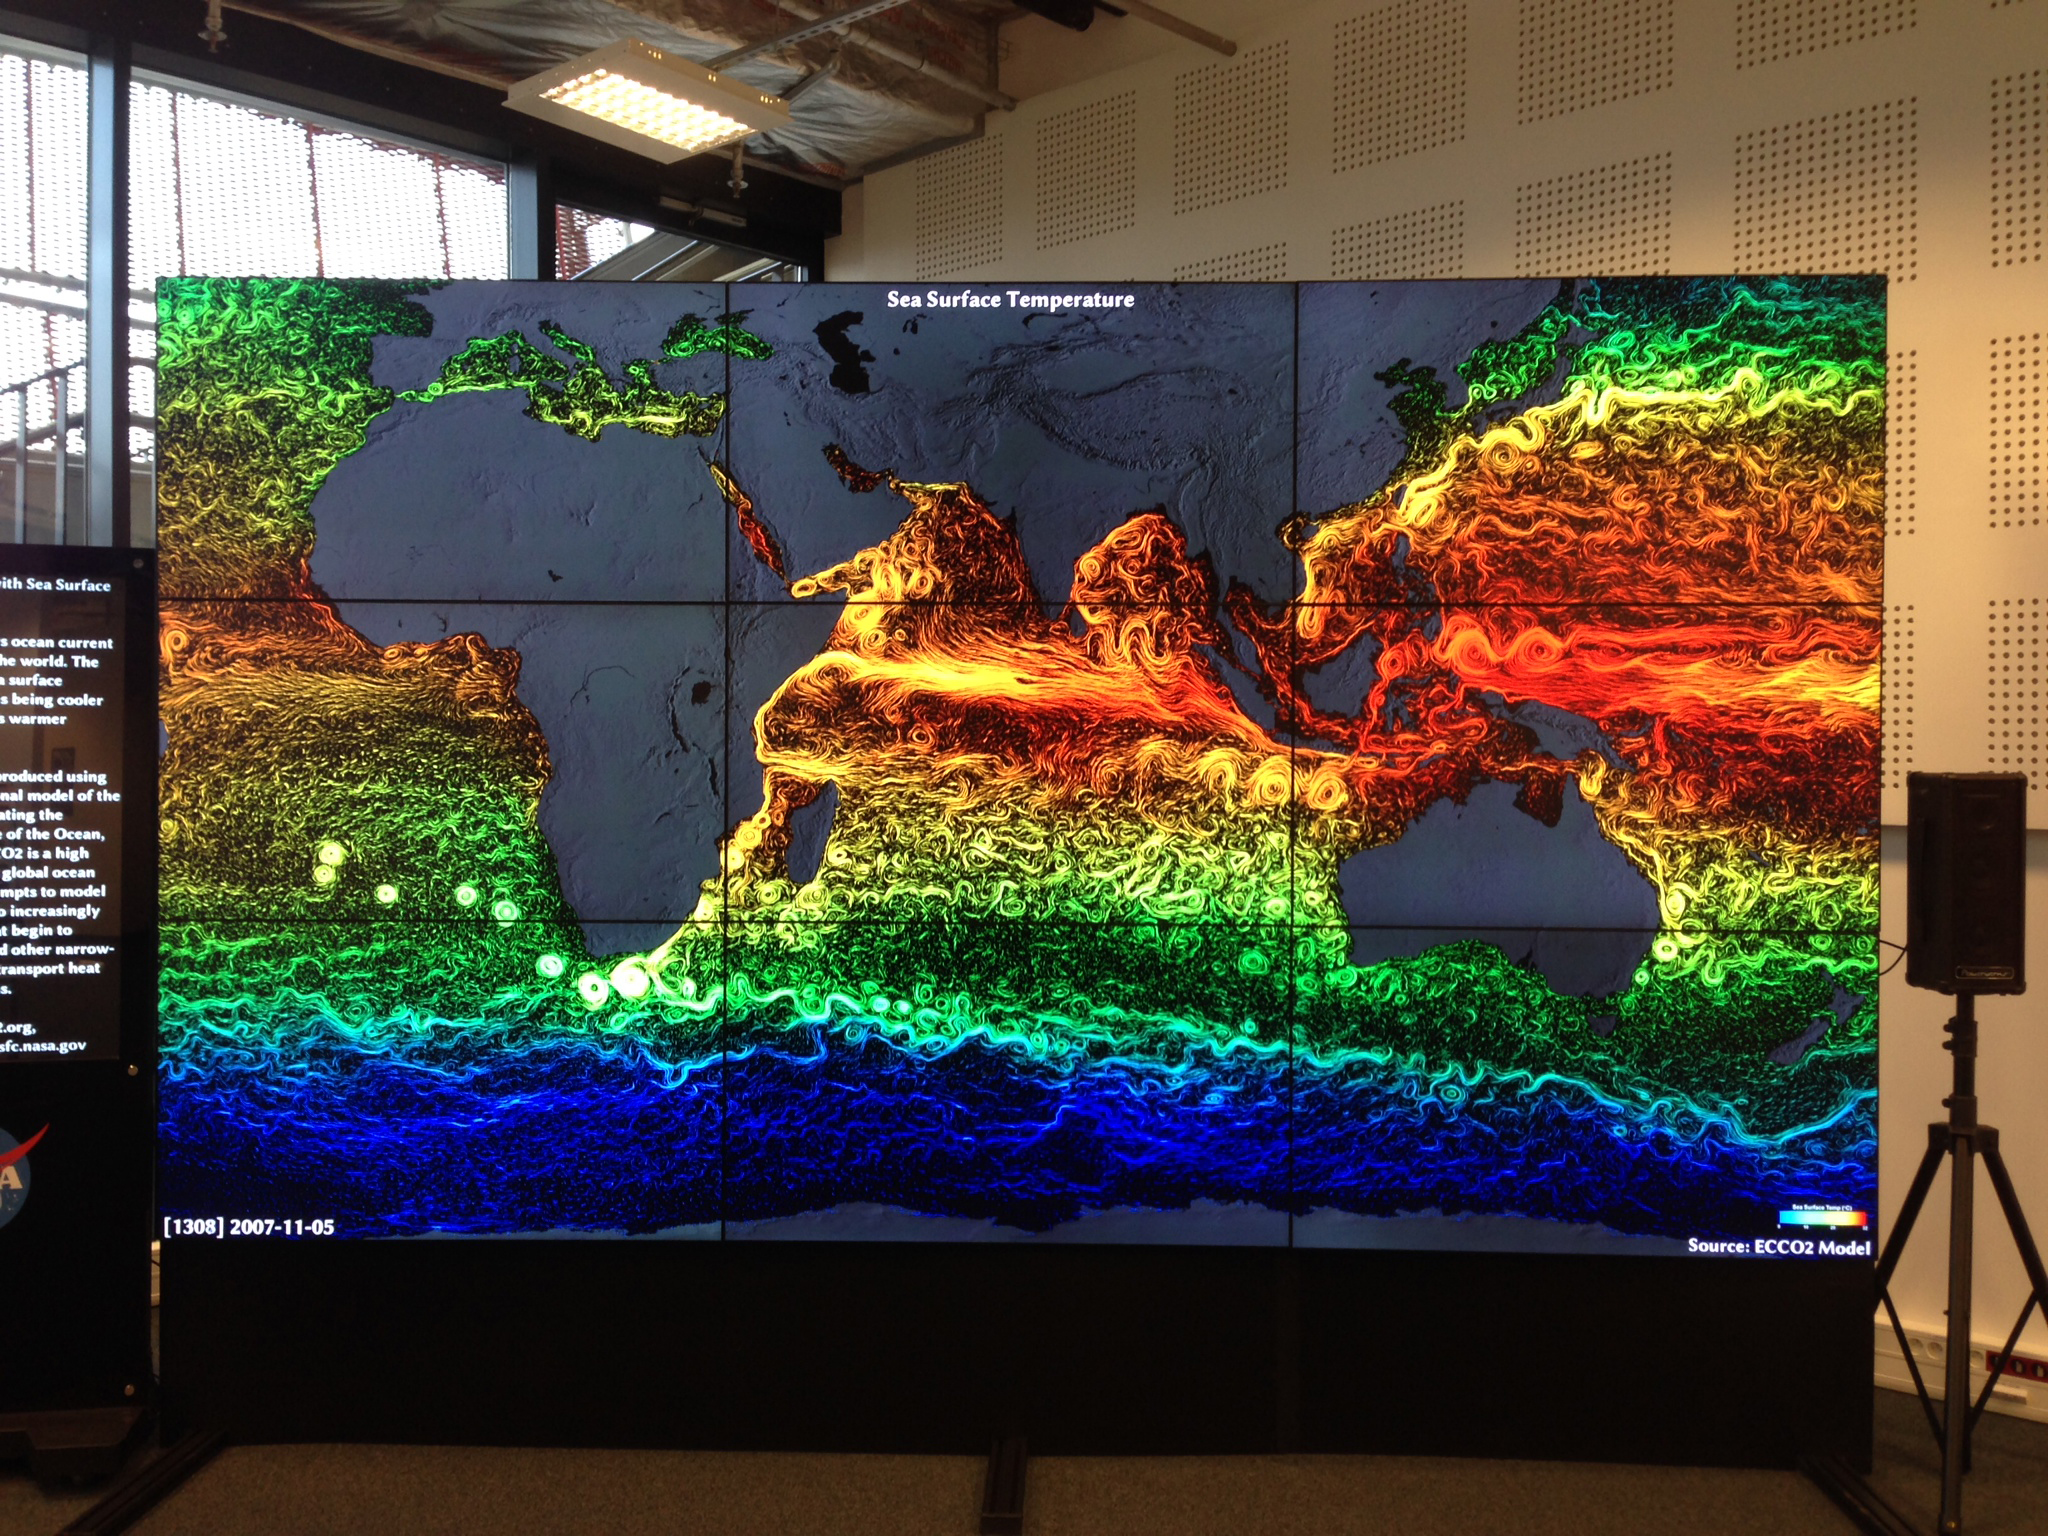
\includegraphics[width=\linewidth,height=91pt,keepaspectratio]{figures/large-display.jpg}\hfil}\vfil}
\smallskip{\scriptsize\sffamily Wall-scale display\par}
\end{minipage}\hfill
\begin{minipage}[t]{0.192\textwidth}\centering
{\small\sffamily\bfseries (c) VR}\par\smallskip
\vbox to 91pt{\vfil\hbox to \linewidth{\hfil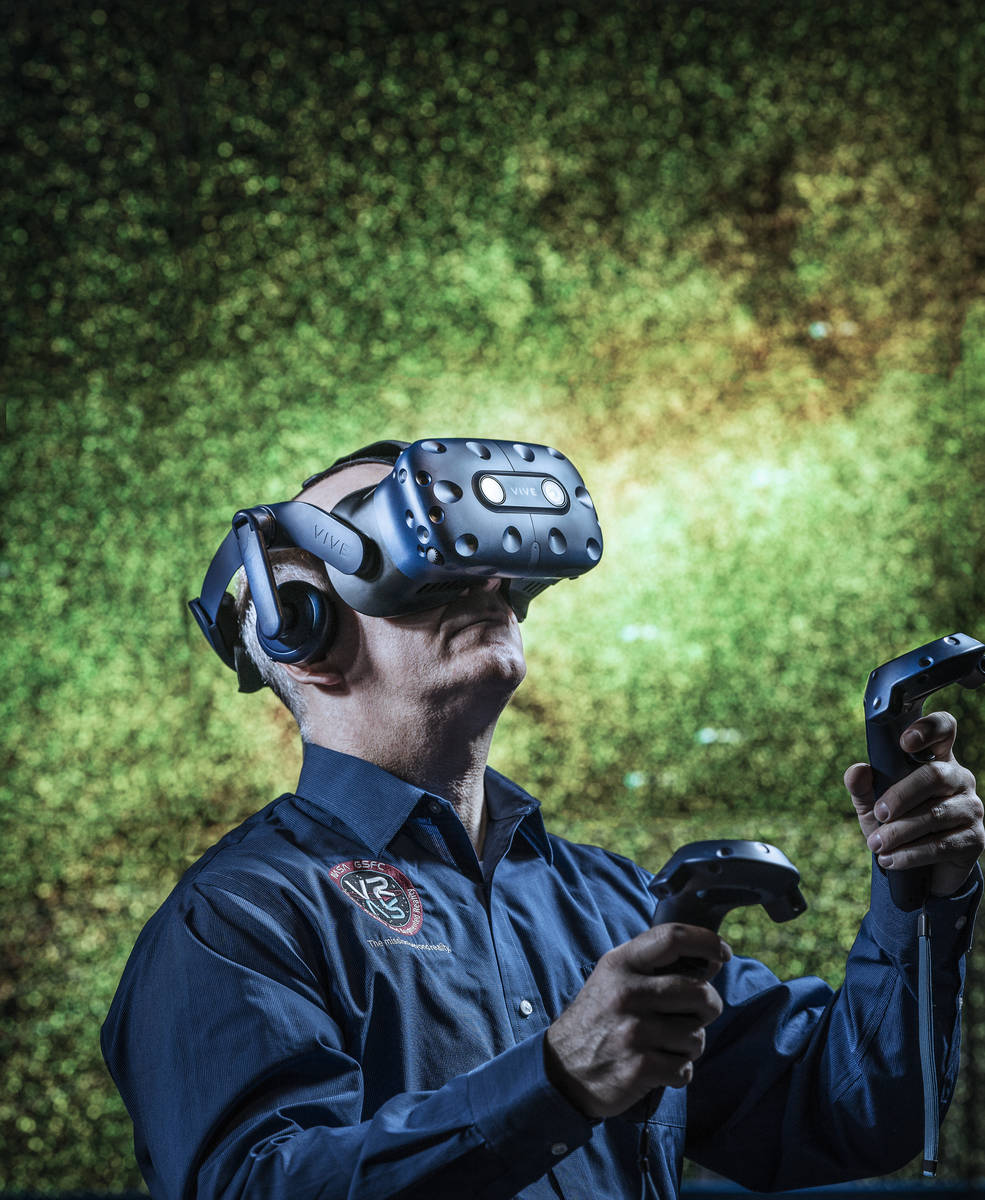
\includegraphics[width=\linewidth,height=91pt,keepaspectratio]{figures/vr.jpg}\hfil}\vfil}
\smallskip{\scriptsize\sffamily Head-mounted virtual scene\par}
\end{minipage}\hfill
\begin{minipage}[t]{0.192\textwidth}\centering
{\small\sffamily\bfseries (d) AR/MR}\par\smallskip
\vbox to 91pt{\vfil\hbox to \linewidth{\hfil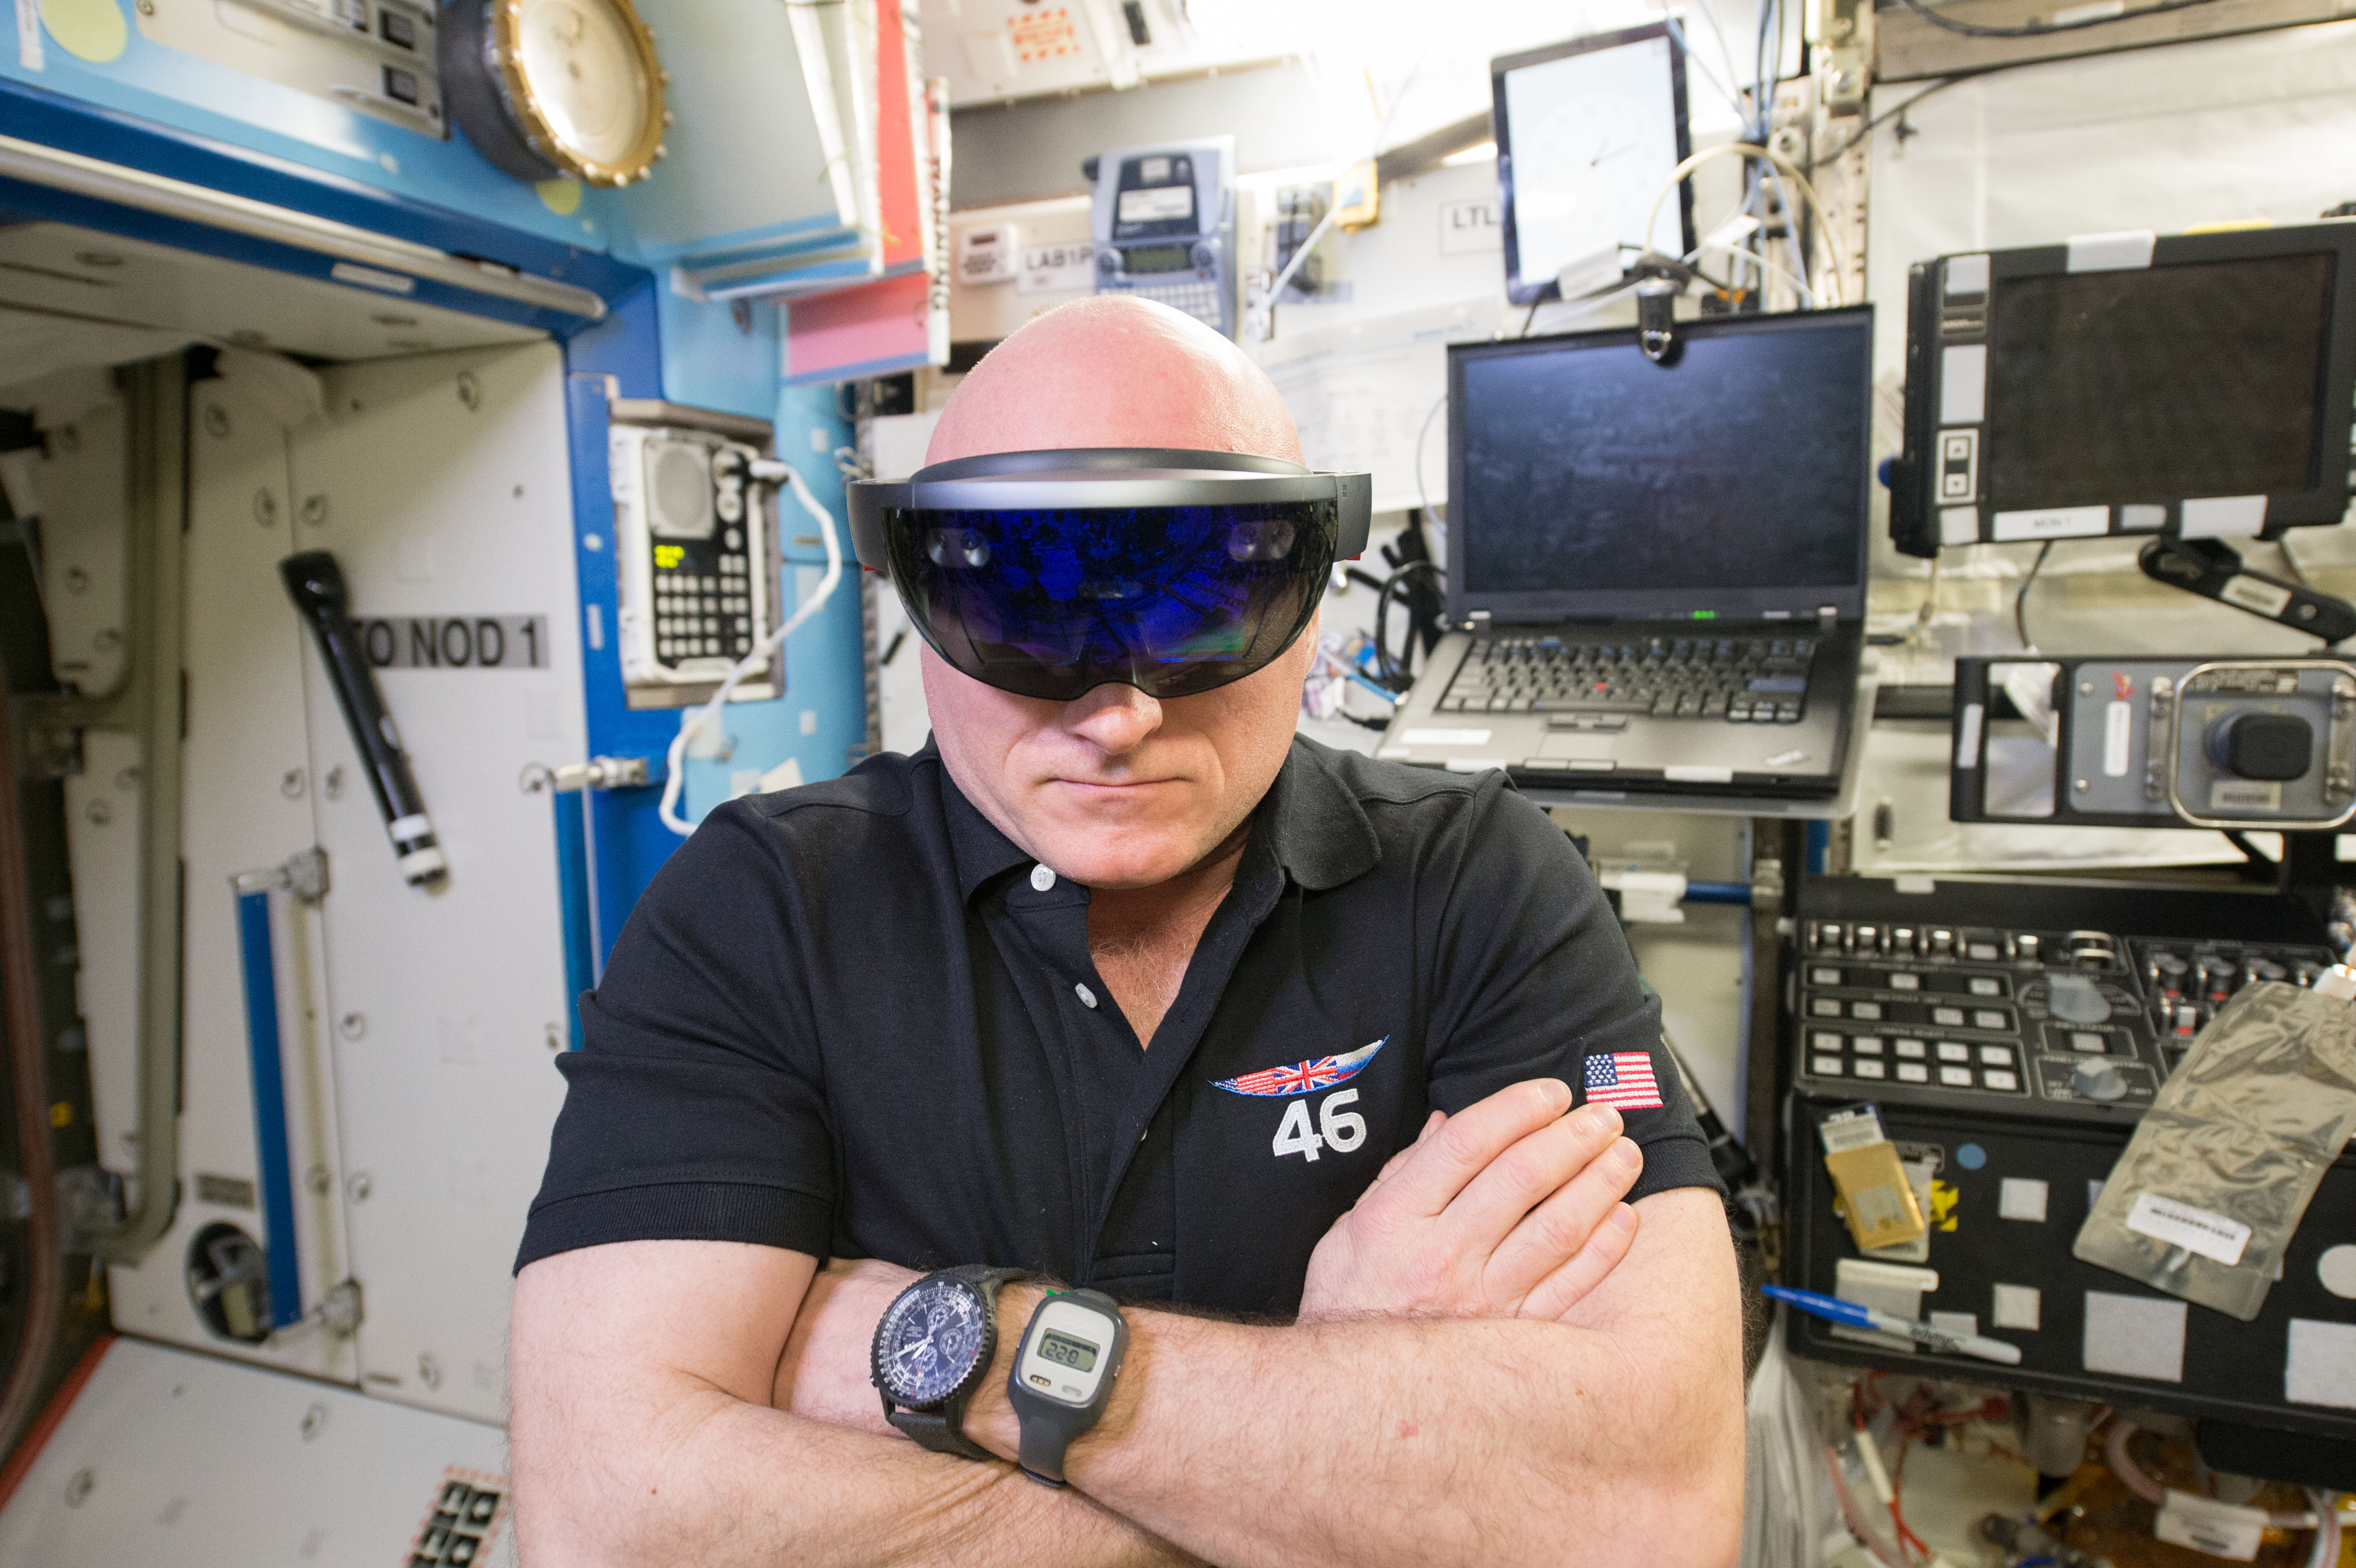
\includegraphics[width=\linewidth,height=91pt,keepaspectratio]{figures/ar-mr.jpg}\hfil}\vfil}
\smallskip{\scriptsize\sffamily Digital + physical context\par}
\end{minipage}\hfill
\begin{minipage}[t]{0.192\textwidth}\centering
{\small\sffamily\bfseries (e) CAVE}\par\smallskip
\vbox to 91pt{\vfil\hbox to \linewidth{\hfil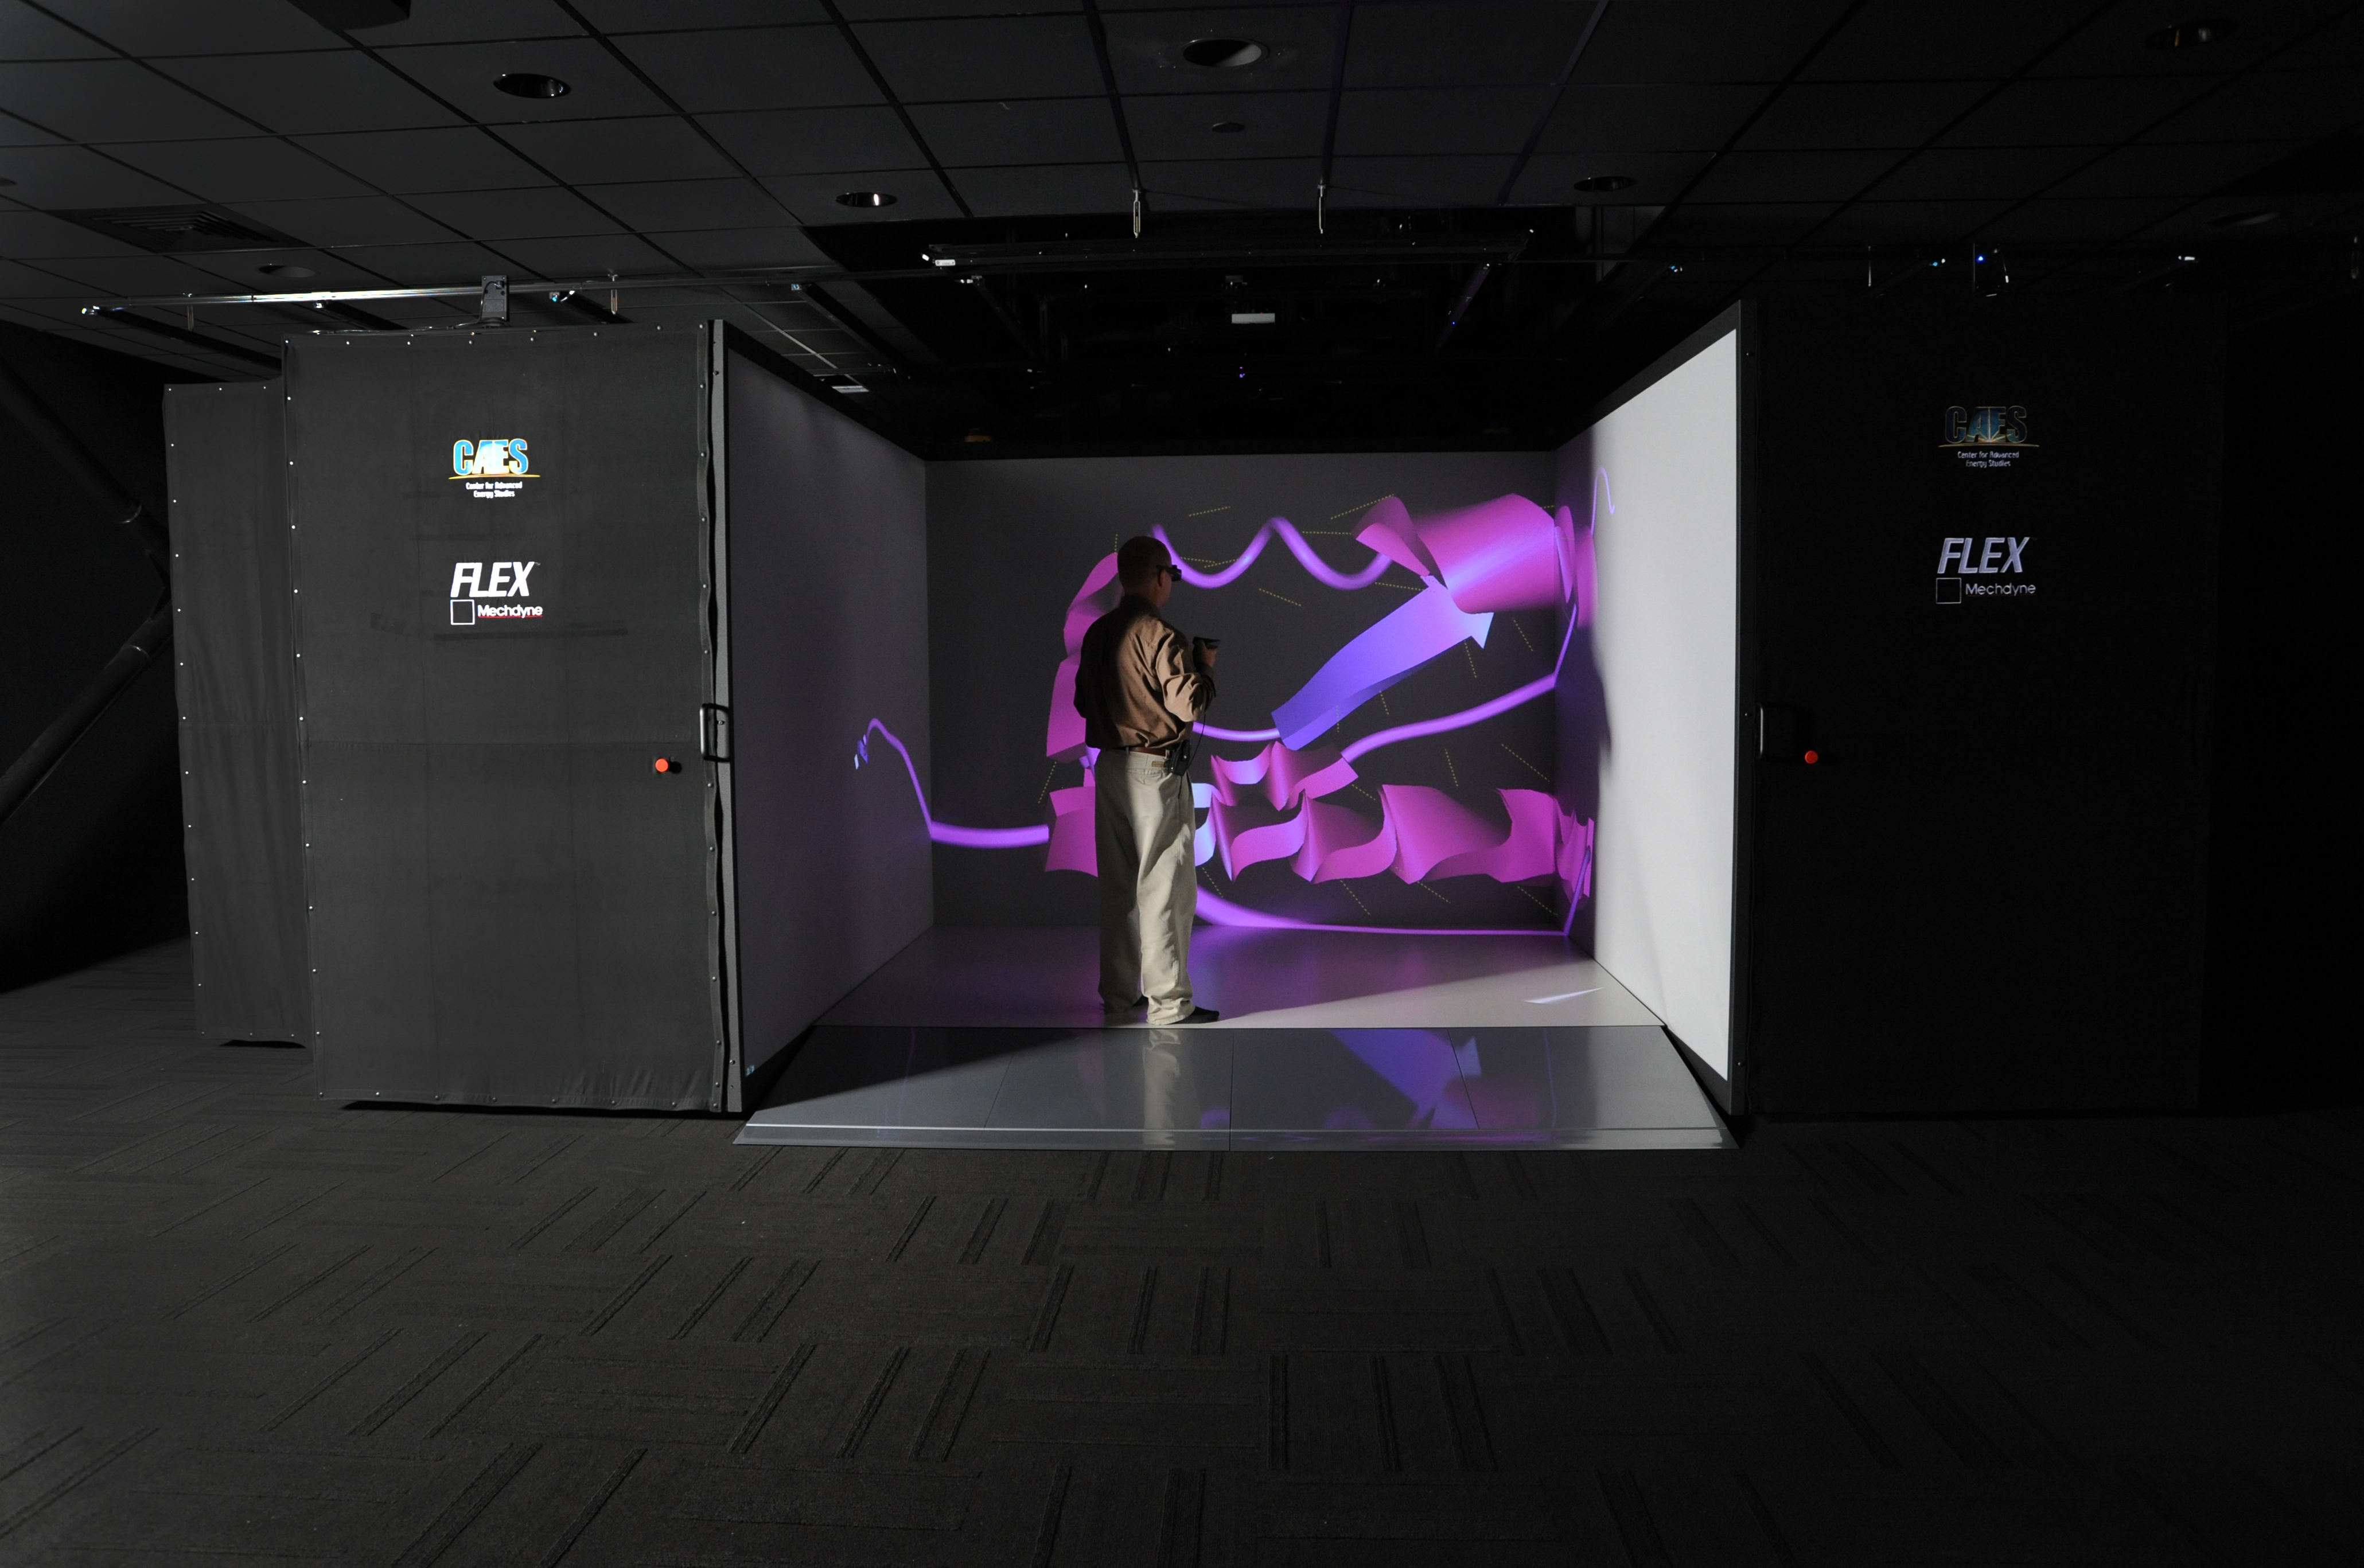
\includegraphics[width=\linewidth,height=91pt,keepaspectratio]{figures/cave.jpg}\hfil}\vfil}
\smallskip{\scriptsize\sffamily Surrounding projections\par}
\end{minipage}
\caption{Examples of the five visualization environments used in this review: (a) a desktop research workstation; (b) NASA's tiled Hyperwall; (c) a virtual-reality headset and controllers; (d) a HoloLens headset used in physical surroundings; and (e) a CAVE displaying a protein model. These photographs illustrate interaction environments, not assistance mechanisms or evidence of analytic benefit. Photographs reproduced without additional cropping: (a) \href{https://commons.wikimedia.org/wiki/File:Scientist_working_with_personal_computer,_2013_(Dell_Precision_T3500_Workstation).jpeg}{Jennie Groom/IPAS (Commons derivative)}, (c) \href{https://commons.wikimedia.org/wiki/File:Exploring_the_Universe_in_Virtual_Reality.jpg}{NASA/Chris Gunn}, and (e) \href{https://commons.wikimedia.org/wiki/File:Cave_automatic_virtual_environment.jpg}{Idaho National Laboratory}, each \href{https://creativecommons.org/licenses/by/2.0/}{CC BY 2.0}; (b) \href{https://commons.wikimedia.org/wiki/File:NASA's_Hyperwall_Shows_the_Sea_Surface_Temperature_(10946045463).jpg}{U.S. Department of State} and (d) \href{https://commons.wikimedia.org/wiki/File:ISS-46_Scott_Kelly_with_HoloLens_in_the_Destiny_lab.jpg}{NASA}, public domain in the United States.}
\label{fig:modality-environments}
\end{figure*}
